\documentclass[11pt]{article}
\usepackage[]{authblk}
\usepackage{graphicx}
\usepackage{color}
\usepackage{longtable}
\usepackage{hanging}
\usepackage{indentfirst}
\usepackage{setspace}
\usepackage{enumitem}
\usepackage{verbatim}
\usepackage{upgreek}
\usepackage{framed}
\usepackage{ textcomp }
\usepackage{url}
\usepackage{soul}
\usepackage{amsmath, amsfonts,amssymb,mathrsfs}
\usepackage{fancyhdr}
\usepackage[compact]{titlesec}
\usepackage[T1]{fontenc}
\usepackage{lmodern}

\usepackage[backend=bibtex,hyperref=true,citestyle=authoryear,bibstyle=authortitle,firstinits=true,terseinits=true,doi=false,url=false,maxbibnames=10,maxcitenames=2]{biblatex}
\addbibresource{../bib_tex/master_refs.bib}
\DeclareCiteCommand{\cite}
  {\usebibmacro{prenote}}
  {\usebibmacro{citeindex}%
   \printtext[bibhyperref]{\usebibmacro{cite}}}
  {\multicitedelim}
  {\usebibmacro{postnote}}

\DeclareCiteCommand*{\cite}
  {\usebibmacro{prenote}}
  {\usebibmacro{citeindex}%
   \printtext[bibhyperref]{\usebibmacro{citeyear}}}
  {\multicitedelim}
  {\usebibmacro{postnote}}

\DeclareCiteCommand{\parencite}[\mkbibparens]
  {\usebibmacro{prenote}}
  {\usebibmacro{citeindex}%
    \printtext[bibhyperref]{\usebibmacro{cite}}}
  {\multicitedelim}
  {\usebibmacro{postnote}}

\DeclareCiteCommand*{\parencite}[\mkbibparens]
  {\usebibmacro{prenote}}
  {\usebibmacro{citeindex}%
    \printtext[bibhyperref]{\usebibmacro{citeyear}}}
  {\multicitedelim}
  {\usebibmacro{postnote}}

\DeclareCiteCommand{\footcite}[\mkbibfootnote]
  {\usebibmacro{prenote}}
  {\usebibmacro{citeindex}%
  \printtext[bibhyperref]{ \usebibmacro{cite}}}
  {\multicitedelim}
  {\usebibmacro{postnote}}

\DeclareCiteCommand{\footcitetext}[\mkbibfootnotetext]
  {\usebibmacro{prenote}}
  {\usebibmacro{citeindex}%
   \printtext[bibhyperref]{\usebibmacro{cite}}}
  {\multicitedelim}
  {\usebibmacro{postnote}}

\DeclareCiteCommand{\textcite}
  {\boolfalse{cbx:parens}}
  {\usebibmacro{citeindex}%
   \printtext[bibhyperref]{\usebibmacro{textcite}}}
  {\ifbool{cbx:parens}
     {\bibcloseparen\global\boolfalse{cbx:parens}}
     {}%
   \multicitedelim}
  {\usebibmacro{textcite:postnote}}

\newcommand{\citep}{\parencite}
\newcommand{\citet}{\textcite}
\defbibheading{relevref}[\refname]{\section*{Relevant References}}

\renewcommand{\postnotedelim}{\iffieldpages{postnote}{\addcolon}{\addcomma\space}} 
\DeclareFieldFormat{postnote}{#1} 

\DeclareFieldFormat[article, inbook, incollection, inproceedings, patent, thesis, unpublished]{title}{#1}
\DeclareFieldFormat[article, inbook, incollection, inproceedings, patent, thesis, unpublished]{journaltitle}{\mkbibemph{#1}\nopunct}
\DeclareFieldFormat[article, inbook, incollection, inproceedings, patent, thesis, unpublished]{volume}{{#1}\addcolon} %puts volume number in parens
%\DeclareFieldFormat[article, inbook, incollection, inproceedings, patent, thesis, unpublished]{year}{\mkbibparens{#1}\nopunct} %puts year in parens

\DeclareFieldFormat[article, incollection, patent, thesis, unpublished]{pages}{{\nopp#1}}

\DeclareFieldFormat{sentencecase}{\MakeSentenceCase{#1}}

\renewbibmacro*{title}{%
  \ifthenelse{\iffieldundef{title}\AND\iffieldundef{subtitle}}
    {}
    {\ifthenelse{\ifentrytype{article}\OR\ifentrytype{inbook}%
      \OR\ifentrytype{incollection}\OR\ifentrytype{inproceedings}%
      \OR\ifentrytype{inreference}}
      {\printtext[title]{%
        \printfield[sentencecase]{title}%
        \setunit{\subtitlepunct}%
        \printfield[sentencecase]{subtitle}}}%
      {\printtext[title]{%
        \printfield[titlecase]{title}%
        \setunit{\subtitlepunct}%
        \printfield[titlecase]{subtitle}}}%
     \newunit}%
  \printfield{titleaddon}}

\DefineBibliographyStrings{english}{% various adjustments to common bib entry strings
urlseen = {Accessed:},% What goes in front of the date a URL was accessed/retrieved etc.
editor = {(Ed)},%Ed – no dot, in brackets
editors = {(Eds)},% Eds – no dot, in brackets
byeditor = {(Ed.)}}% ‘Edited by’ for edited works

\DeclareNameAlias{default}{last-first}

\renewbibmacro{in:}{}

\renewbibmacro{publisher+location+date}{
  \iflistundef{publisher}
    {}
    {\printlist{publisher}%
       {\addcomma\space}%
      \iflistundef{location}
        {}
        {\printlist{location}}%
    }
}

\DeclareBibliographyDriver{article}{%
\usebibmacro{bibindex}%
\usebibmacro{begentry}%
\usebibmacro{author/translator+others}%
\newunit\newblock
\printfield{year}%
\setunit{\labelnamepunct}\newblock
\usebibmacro{title}%
\newunit
\printlist{language}%
\newunit\newblock
\usebibmacro{byauthor}%
\newunit\newblock
\usebibmacro{bytranslator+others}%
\newunit\newblock
\printfield{version}%
\newunit\newblock
%\usebibmacro{in:}% %mit in:
\usebibmacro{journal}%
\newunit\newblock
\printfield{volume}%
\newunit\newblock
\usebibmacro{byeditor+others}%
\newunit\newblock
\usebibmacro{note+pages}%
\newunit\newblock
\iftoggle{bbx:isbn}
{}%
\newunit\newblock
\usebibmacro{doi+eprint+url}%
\newunit\newblock
\usebibmacro{addendum+pubstate}%
\newunit\newblock
\usebibmacro{pageref}%
\usebibmacro{finentry}}

\DeclareBibliographyDriver{inproceedings}{%
\usebibmacro{bibindex}%
\usebibmacro{begentry}%
\usebibmacro{author/translator+others}%
\newunit\newblock
\printfield{year}%
\setunit{\labelnamepunct}\newblock
\usebibmacro{title}%
\newunit
\printlist{language}%
\newunit\newblock
\usebibmacro{byauthor}%
\newunit\newblock
\usebibmacro{bytranslator+others}%
\newunit\newblock
\printfield{version}%
\newunit\newblock
%\usebibmacro{in:}% %mit in:
\usebibmacro{booktitle}%
\newunit\newblock
\printfield{volume}%
\newunit\newblock
\usebibmacro{byeditor+others}%
\newunit\newblock
\usebibmacro{publisher+location+date}%
\newunit\newblock
\usebibmacro{note+pages}%
\newunit\newblock
\usebibmacro{pageref}%
\usebibmacro{finentry}}

\DeclareBibliographyDriver{book}{%
\usebibmacro{bibindex}%
\usebibmacro{begentry}%
\usebibmacro{author/translator+others}%
\newunit\newblock
\printfield{year}%
\setunit{\labelnamepunct}\newblock
\usebibmacro{title}%
\newunit
\printlist{language}%
\newunit\newblock
\usebibmacro{byauthor}%
\newunit\newblock
\usebibmacro{bytranslator+others}%
\newunit\newblock
%\usebibmacro{in:}% %mit in:
\usebibmacro{booktitle}%
\newunit\newblock
\printfield{volume}%
\newunit\newblock
\usebibmacro{publisher+location+date}%
\newunit\newblock
\usebibmacro{note+pages}%
\newunit\newblock
\usebibmacro{pageref}%
\usebibmacro{finentry}}





\setlength{\evensidemargin}{0in}
\setlength{\headheight}{0in}
\setlength{\headsep}{0in}
\setlength{\oddsidemargin}{-0.25in}
\setlength{\paperheight}{11in}
\setlength{\paperwidth}{8.5in}
\setlength{\tabcolsep}{0in}
\setlength{\textheight}{9in}
\setlength{\textwidth}{7in}
\setlength{\topmargin}{0in}
\setlength{\topskip}{0in}
\setlength{\voffset}{0in}
\parskip = 0.15in
\pagestyle{plain}
\setlength{\parindent}{0cm}

\definecolor{citescol}{RGB}{194,101,1}
\definecolor{urlscol}{RGB}{0,150,206}
\definecolor{linkscol}{RGB}{149,0,207}
\definecolor{mycol}{RGB}{25,23,191}
\definecolor{outputcol}{RGB}{34,139,34}
\definecolor{tcol}{RGB}{165,0,14}


\DeclareMathAlphabet{\msfsl}{T1}{cmr}{m}{it}
\DeclareMathAlphabet{\msyf}{OMX}{pcr}{m}{it}
\newcommand{\alf}{\upalpha}
\newcommand{\hilight}[1]{\colorbox{yellow}{#1}}

\newcommand{\levelone}[1]{
\bigskip
\noindent{\LARGE{\textsc{#1}}}
\vspace {0.05in}
}

\newcommand{\leveltwo}[1]{
\bigskip
\noindent{\Large{\textit{#1}}}
\vspace {-1mm}
}

\newcommand{\descriptionhead}[1]{
\noindent{\textbf{\textit{#1}}}\\ \vspace{-7mm}
}

\newcommand{\dhead}[1]{
\noindent{\textbf{\textit{#1 --}}}
}


\newcommand{\exs}[1]{
\vspace{-4mm}
\begin{itemize}
\item #1 \\ \vspace{-8mm}
\end{itemize}
}

\newcommand{\nbo}[1]{{\color{red}{#1}}}


\newcommand{\stepbullet}{\noindent \textbullet \ }
\newcommand{\mi}[1]{\textbf{\textit{#1}}}


\newcommand{\levelthree}[1]{\textit{#1 --}}


%\bibliographystyle{apalike}
%\bibpunct[; ]{(}{)}{;}{a}{,}{;}


\usepackage[breaklinks]{hyperref}
\usepackage[all]{hypcap}
\hypersetup{colorlinks=true,linkcolor=linkscol,citecolor=citescol,urlcolor=urlscol}


\newcommand{\R}{\texttt{R} }
\newcommand{\TESS}{\texttt{TESS}}
\newcommand{\PBD}{\texttt{PBD}}
\newcommand{\DDD}{\texttt{DDD}}
\newcommand{\Laser}{\texttt{laser}}
\newcommand{\TreePar}{\texttt{TreePar}}
\newcommand{\diversitree}{\texttt{diversitree}}
\newcommand{\RevBayes}{\texttt{RevBayes}}
\newcommand{\Rev}{\texttt{Rev}}
\newcommand{\MrBayes}{\texttt{MrBayes}}
\newcommand{\BEAST}{\texttt{BEAST}}
\newcommand{\PhyloBayes}{\texttt{PhyloBayes}}
\newcommand{\PAML}{\texttt{PAML}}

\let\otheriint\iint
\let\iint\relax
\usepackage{ wasysym }

\usepackage{framed}
\usepackage[]{listings}
%\usepackage{fontspec}
\usepackage{placeins}
\usepackage{epstopdf}

\lstset{breaklines=true}

\definecolor{shadecolor}{RGB}{238,224,229}

\setlength{\tabcolsep}{5pt}
\setlength{\topmargin}{-0.4in}
\setlength{\headheight}{14.5pt}
\pagestyle{fancy}

\newcommand{\taha}[1]{{\textcolor{red}{[TAH comment: #1]}}} % TAH comment

\titlespacing{\section}{0pt}{*0}{*0}
\titlespacing{\subsection}{0pt}{*0}{*0}
\titlespacing{\subsubsection}{0pt}{*0}{*0}

\titleformat{\section}
  {\normalfont\Large\bfseries\color{mycol}}
  {\thesection}{1em}{}

\titleformat{\subsection}
  {\normalfont\large\bfseries\color{mycol}}
  {\thesubsection}{1em}{}

\titleformat{\subsubsection}
  {\normalfont\bfseries\color{mycol}}
  {\thesubsubsection}{1em}{}

% command for MrBayes command-line step
\newcommand{\cl}[1]{{\texttt{\textbf{#1}}}}

\newcommand{\colx}[1]{{\textcolor{tcol}{#1}}}

\newcommand{\mbcl}[1]{\exs{\cl{MrBayes > {#1}}}}

\newcommand{\rbprmt}{RevBayes > } 
\newcommand{\rbcl}[1]{\exs{\cl{\rbprmt{#1}}}}
\newcommand{\rbout}[1]{\exs{\cl{\textcolor{outputcol}{#1}}}}
\newcommand{\rbdn}{{\Large \symbol{126}}} % This makes a copy/pasteable tilde
\newcommand{\rbclml}[1]{\exs{\cl{\ \ \ \ \ \ \ \ \ \ \ {#1}}}}

% text box settings
% requires compiling w/ XeLaTeX
%\newfontfamily\listingsfont[Scale=1.0]{Courier New}
%\lstset{basicstyle=\listingsfont, columns=texcl}
%\defaultfontfeatures{Mapping=tex-text}


\makeatletter
\lst@CCPutMacro\lst@ProcessOther {"2D}{\lst@ttfamily{-{}}{-{}}}
\@empty\z@\@empty
\makeatother


\usepackage{framed}
\usepackage[]{listings}
\usepackage{fontspec}
\usepackage{placeins}
\usepackage{epstopdf}

\lstset{breaklines=true}

\definecolor{shadecolor}{RGB}{238,224,229}


\setlength{\topmargin}{-0.4in}
\setlength{\headheight}{14.5pt}
\pagestyle{fancy}

\newcommand{\taha}[1]{{\textcolor{red}{[TAH comment: #1]}}} % TAH comment

\titlespacing{\section}{0pt}{*0}{*0}
\titlespacing{\subsection}{0pt}{*0}{*0}
\titlespacing{\subsubsection}{0pt}{*0}{*0}

\titleformat{\section}
  {\normalfont\Large\bfseries\color{mycol}}
  {\thesection}{1em}{}

\titleformat{\subsection}
  {\normalfont\large\bfseries\color{mycol}}
  {\thesubsection}{1em}{}

\titleformat{\subsubsection}
  {\normalfont\bfseries\color{mycol}}
  {\thesubsection}{1em}{}

% command for MrBayes command-line step
\newcommand{\cl}[1]{{\texttt{\textbf{#1}}}}

\newcommand{\colx}[1]{{\textcolor{tcol}{#1}}}

\newcommand{\mbcl}[1]{\exs{\cl{MrBayes > {#1}}}}

\newcommand{\rbprmt}{RevBayes > } 
\newcommand{\rbcl}[1]{\exs{\cl{\rbprmt{#1}}}}
\newcommand{\rbout}[1]{\exs{\cl{\textcolor{outputcol}{#1}}}}
\newcommand{\rbdn}{{\Large \symbol{126}}} % This makes a copy/pasteable tilde
\newcommand{\rbclml}[1]{\exs{\cl{\ \ \ \ \ \ \ \ \ \ \ {#1}}}}

% text box settings
% requires compiling w/ XeLaTeX
\newfontfamily\listingsfont[Scale=1.0]{Courier New}
\lstset{basicstyle=\listingsfont, columns=texcl}
\defaultfontfeatures{Mapping=tex-text}


\makeatletter
\lst@CCPutMacro\lst@ProcessOther {"2D}{\lst@ttfamily{-{}}{-{}}}
\@empty\z@\@empty
\makeatother

\begin{document}
\renewcommand{\headrulewidth}{0.5pt}
\headsep = 20pt
\lhead{ }
\rhead{\textsc {RevBayes Tutorial --- Model Selection \& Partitioning}}

\thispagestyle{plain}
\begin{center}

\textbf{\LARGE Phylogenetic Inference using RevBayes}\\\vspace{2mm}
\textbf{\it{\Large Model Selection \& Data Partitioning}}\\\vspace{2mm}
\end{center}

\section*{Overview}

RevBayes has as a central idea that phylogenetic models, like any statistical model, are composed of smaller parts that can be decomposed and 
put back together in a modular fashion. This comes from considering phylogenetic models as \textit{probabilistic graphical models}, 
which lends flexibility and enhances the capabilities of the program. 
RevBayes implements an R-like language (complete with control statements, user-defined functions, and loops) 
that enables the user to build up phylogenetic models from simple parts (random variables, transformations, models, 
and constants of different sorts).
%RevBayes is a software program for inferring phylogenetic parameters in a Bayesian statistical framework. 
%RevBayes is ``descended'' from MrBayes \citep{huelsenbeck01c,ronquist03,huelsenbeck05,Ronquist2012}, which has been (and still is) one of the most commonly used Bayesian phylogenetic inference programs. 
%However, RevBayes is a complete rewrite and a very different approach to the engineering of the program was taken. 
%
%RevBayes uses \textit{probabilistic graphical models} for model specification and implementation \citep{hoehnaGM2014}. 
%This framework is common in the fields of statistics and machine learning to represent complex  statistical models with many parameters \citep{Gilks1994,lunn00,Jordan2004,Koller2009,Lunn2009}. 
%The graphical model tool kit allows for flexible model specification and implementation and reduces redundant code. 
%This approach to statistical inference requires a rich programming language and interface to define models and analysis details. 
%Thus, RevBayes also 

%RevBayes and the Rev language are still under active development. Thus, this tutorial comes with some caveats. First, there are many methods currently available in RevBayes, but many more that are not yet fully implemented. 
 

This tutorial demonstrates how to set up and perform an analysis that calculates Bayes factors to select among different 
partition configurations of aligned DNA sequences. 
After selecting the model that is best supported by the data, the exercise continues with basic inference of an unrooted 
tree topology and branch lengths using Markov chain Monte Carlo (MCMC). 


\bigskip
\subsection{Probabilistic Graphical Models}

RevBayes uses \textit{probabilistic graphical models} for model specification, visualization, and implementation \citep{hoehnaGM2014}. 
Graphical models are frequently used in machine learning and statistics to visually represent the conditional dependence 
structure of complex statistical models with many parameters \citep{Gilks1994,lunn00,Jordan2004,Koller2009,Lunn2009}. 
The graphical model tool kit allows for flexible model specification and implementation and reduces redundant code. 
This framework provides a set of symbols for depicting a \href{http://en.wikipedia.org/wiki/Directed_acyclic_graph}{\textit{directed acyclic graph}} (DAG). 
\citet{hoehnaGM2014} described the use of probabilistic graphical models for phylogenetics. 
The different nodes and components of a phylogenetic graphical model are shown in Figure \ref{gmnotation} \citep[Fig. 1 from][]{hoehnaGM2014}. 
\begin{figure}[h!]
\centering
\fbox{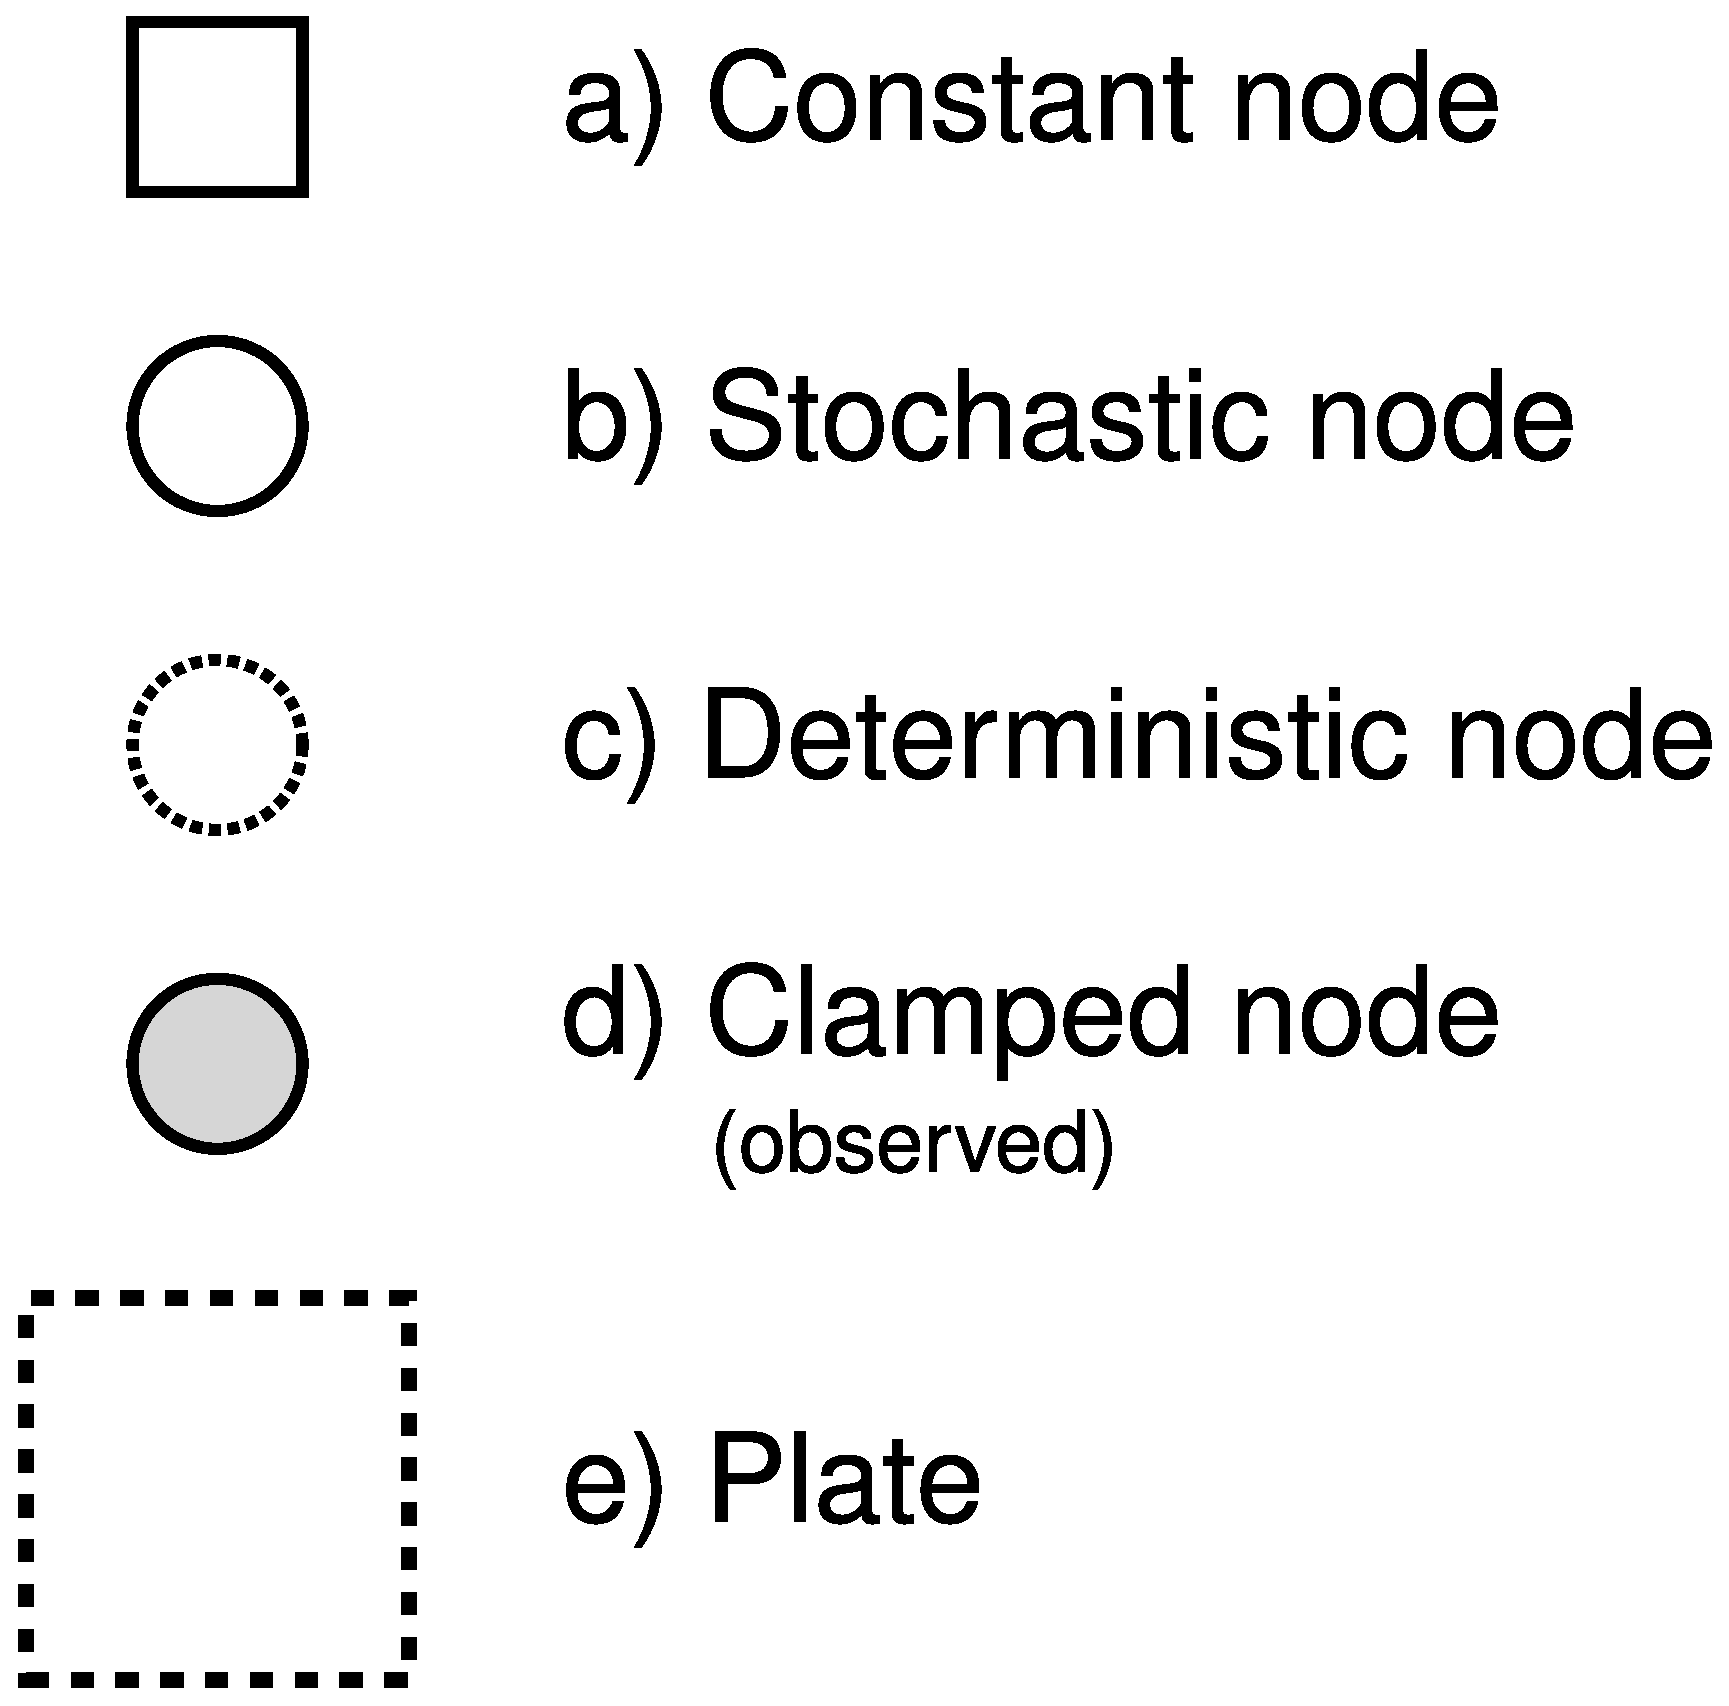
\includegraphics[width=1.8in,angle=0]{figures/GM_notation_figure.eps}}
\caption{\small The symbols for a visual representation of a graphical model. a) Solid squares represent constant nodes, 
which specify fixed-valued variables. b) Stochastic nodes are represented by solid circles. 
These variables correspond to random variables and may depend on other variables. c) Deterministic nodes (dotted circles) 
indicate variables that are determined by a specific function applied to another variable. 
They can be thought of as variable transformations. d) Observed states are placed in clamped stochastic nodes, 
represented by gray-shaded circles. e) Replication over a set of variables is indicated by enclosing the replicated nodes 
in a plate (dashed rectangle). [Replicated from Fig.~1 in \citet{hoehnaGM2014}.]}
\label{gmnotation}
\end{figure}

To represent the DAG, nodes are connected with arrows indicating dependency. 
A simple, albeit abstract, graphical model is shown in Figure \ref{simpleGM}. 
In this model, we observe a set of states for parameter $x$. 
We assume that the values of $x$ are samples from a lognormal distribution with a location parameter (log mean) 
$\mu$ and a standard deviation $\sigma$. 
It is more straightforward to model our uncertainty in the expectation of a lognormal distribution, rather than $\mu$, 
thus we place a gamma distribution on the mean $M$. This gamma hyperprior has two parameters that we specify with fixed 
values (constant nodes): the shape $\alpha$ and rate $\beta$. 
With this prior density, the variable $M$ is a stochastic node.
The standard deviation, $\sigma$, is also a stochastic node with an exponential prior density with rate parameter $\lambda$.
For any value of $M$ and any value of $\sigma$ we can compute the deterministic variable $\mu$ using the formula 
$\mu = \ln(M) - \frac{\sigma^2}{2}$. 
This formula is known from using simple algebra on the equation for the mean of any \href{http://en.wikipedia.org/wiki/Log-normal_distribution}{lognormal distribution}.
With this model structure, we can then calculate the probability of the data conditional on the model (the likelihood): 
$\mathbb{P}(\boldsymbol{x} \mid \mu, \sigma)$. With this, we can get the posterior probability using Bayes' theorem:
$$\mathbb{P}(M,\sigma \mid \boldsymbol{x}, \alpha, \beta, \lambda) = \frac{\mathbb{P}(\boldsymbol{x} \mid \mu, \sigma) \mathbb{P}(M \mid \alpha,\beta) \mathbb{P}(\sigma \mid \lambda)}{\mathbb{P}(\boldsymbol{x})}.$$
\begin{figure}[h!]
\centering
\fbox{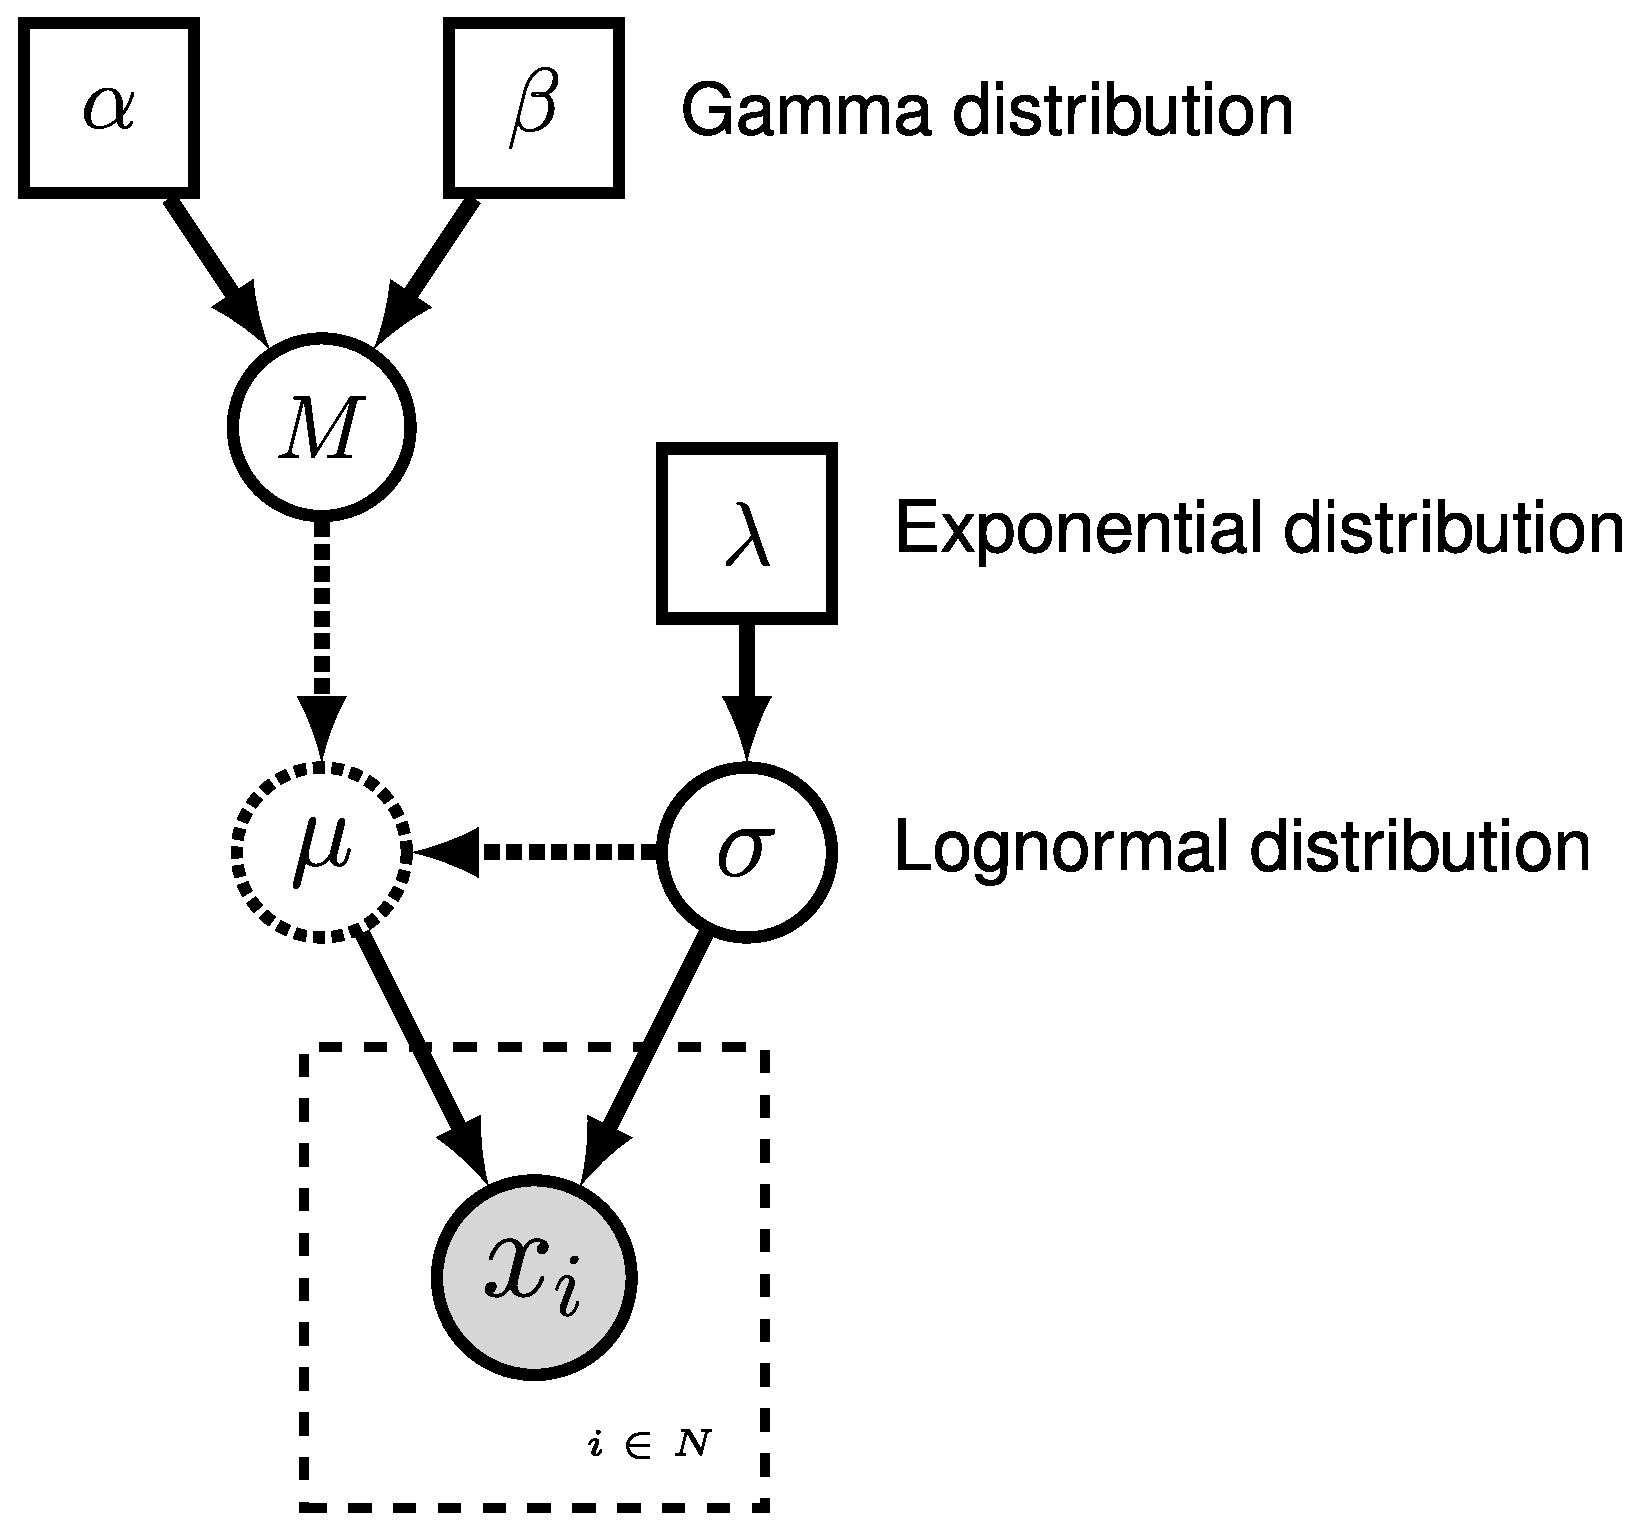
\includegraphics[width=2.5in,angle=0]{figures/simple_GM.eps}}
\caption{\small Graphical model representation of a simple lognormal model. A total of $N$ states of parameter $x$ are observed and occupy a clamped node. This parameter is log-normally 
distributed with parameters $\mu$ and $\sigma$ (log mean and standard deviation, respectively). The parameter $\mu$ is a 
deterministic node that is calculated from the stochastic nodes $M$ (the mean of the distribution) and $\sigma$. 
Dotted arrows indicate deterministic functions and are used to connect deterministic nodes to their parent variables. 
A gamma distribution is applied as a hyper prior on $M$ with constant nodes for the shape $\alpha$ and rate $\beta$. 
The stochastic variable $\sigma$ is exponentially distributed with fixed value for the rate $\lambda$.}
\label{simpleGM}
\end{figure}

For phylogenetic graphical model representations, \citet{hoehnaGM2014} introduced a new element called the \textit{tree plate}. 
This is a convenience for visualization because, although a phylogenetic tree is a graphical model, the complexity becomes intractable for large trees. 
Thus, the tree plate depicts replication over a given topology. 
The full graphical model with the unrooted tree plate for the GTR$+\Gamma$ model used in this tutorial is shown in Figure \ref{gtrgmfig}. Note that even unrooted analyses arbitrarily assign a root node to orient the tree.
\begin{figure}[h!]
\centering
\fbox{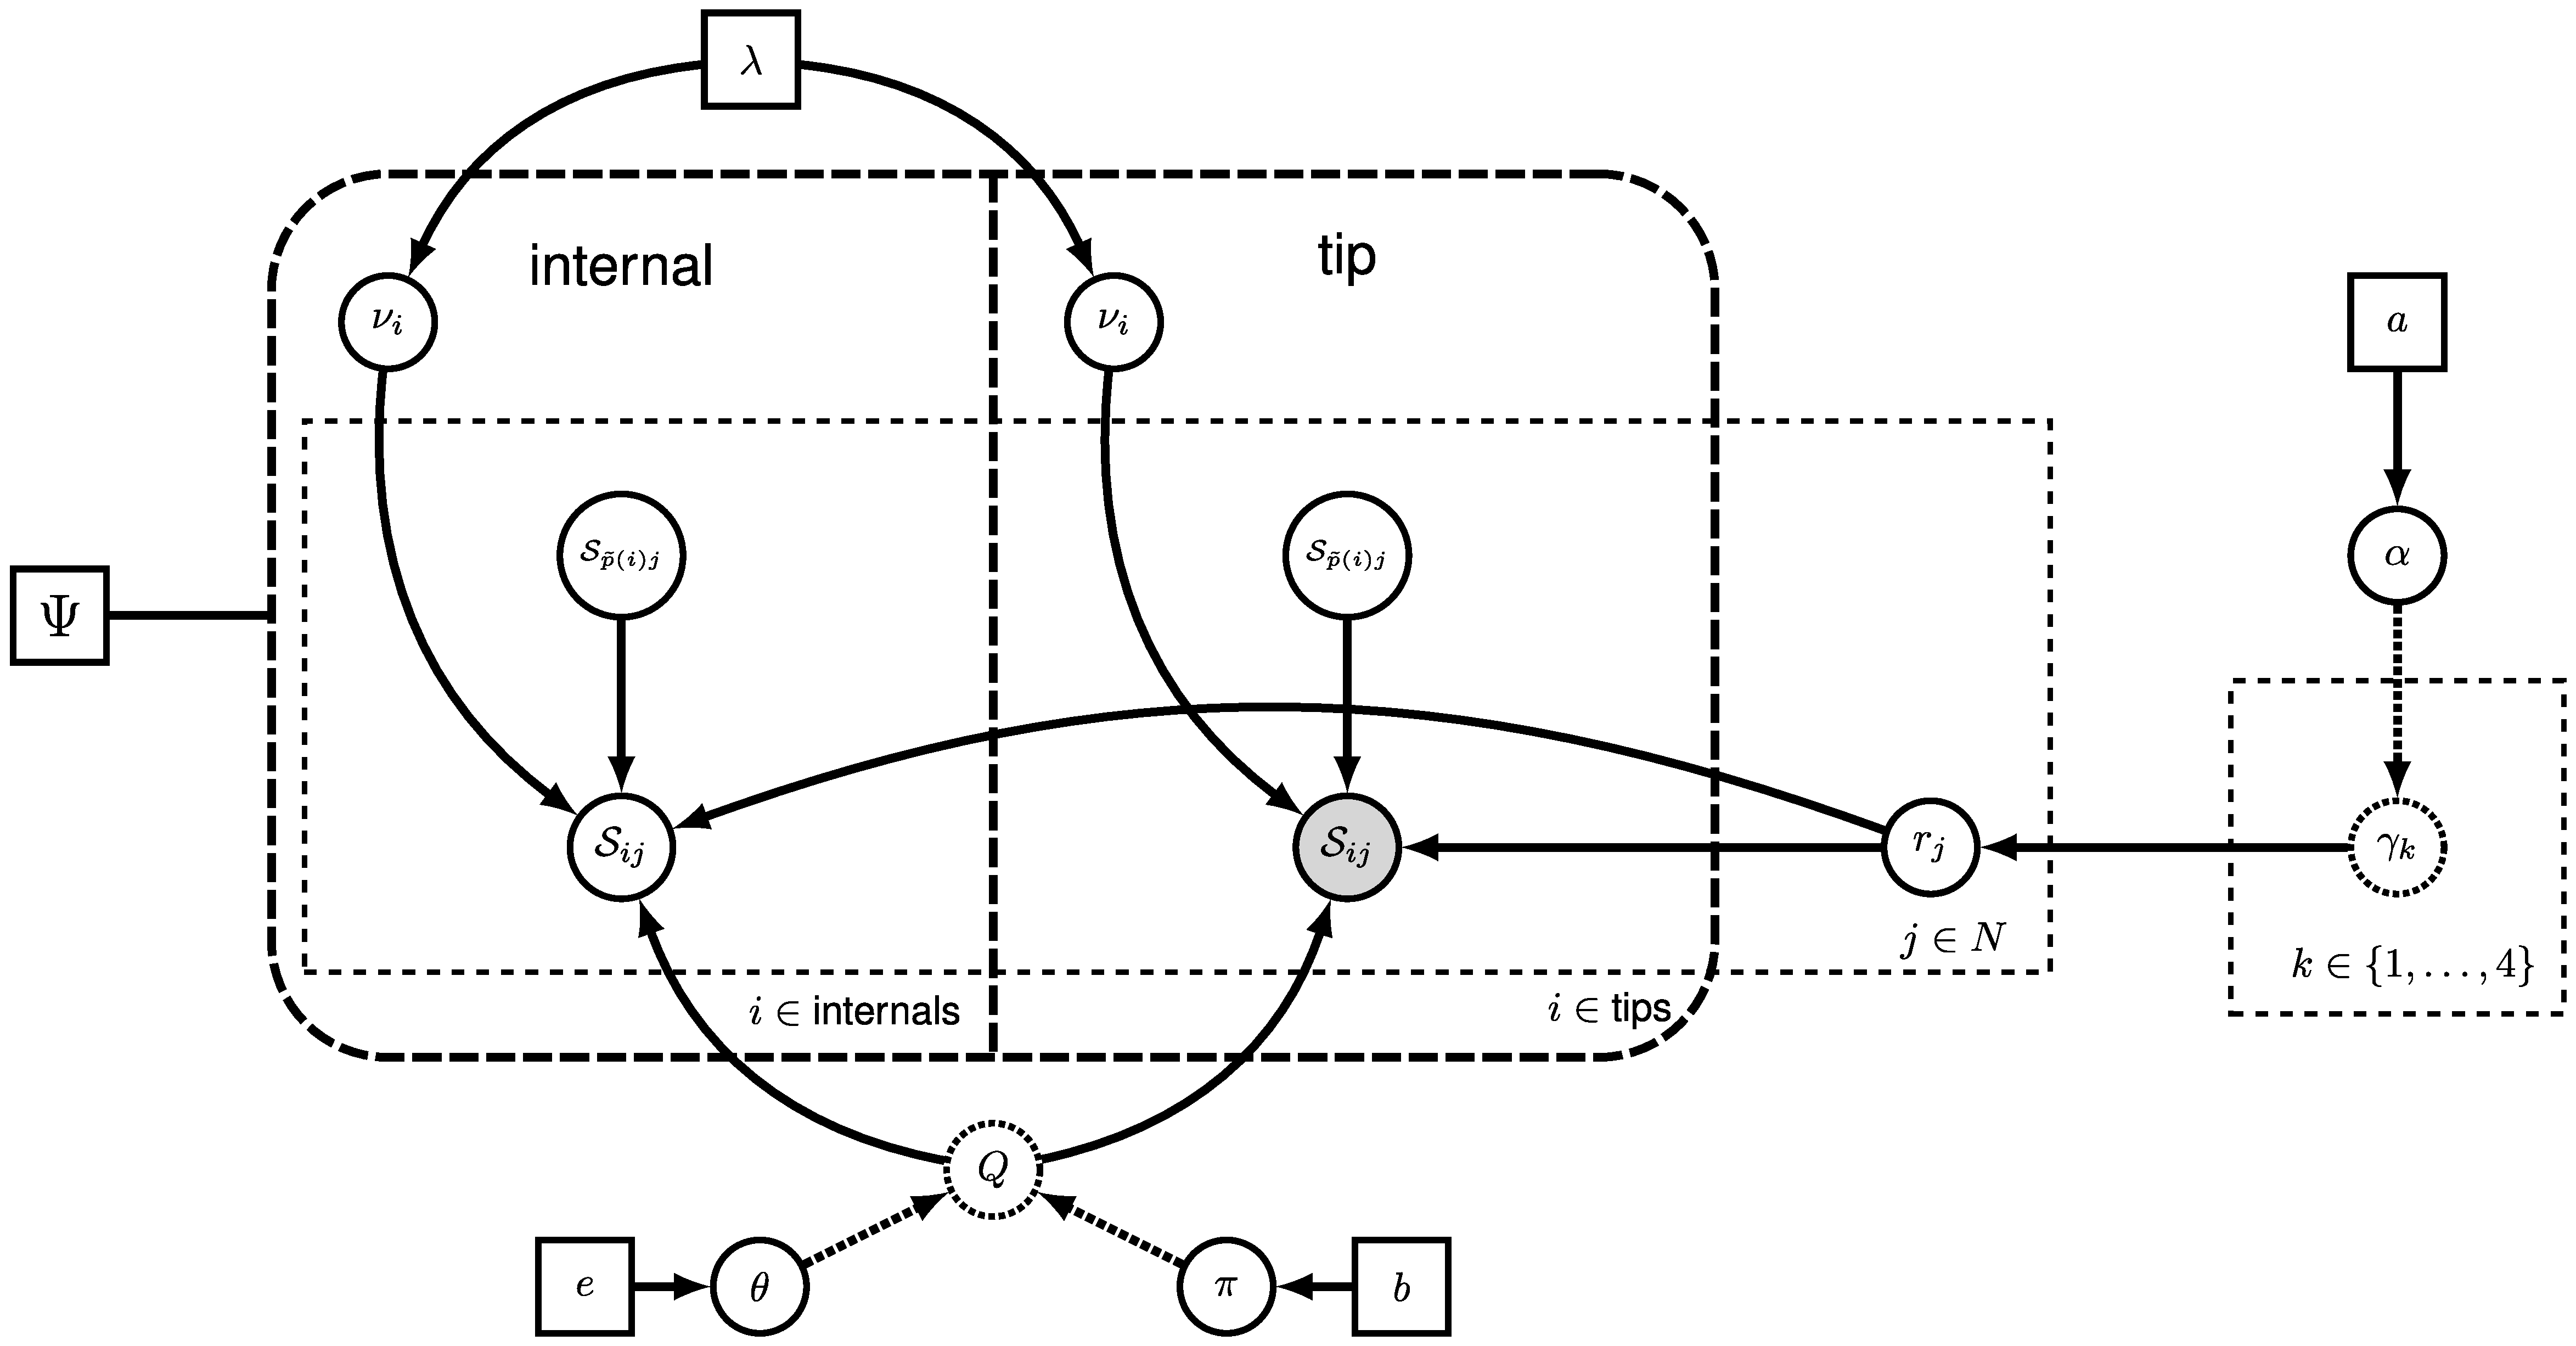
\includegraphics[width=6.8in,angle=0]{figures/gtrg_graphical_model}}
\caption{\small  The general-time reversible model \citep{tavare86} with gamma-distributed rate variation across sites \citep{yang94a}: GTR$+\Gamma$. 
The tree plate separates the nodes of the tree into different categories. For any tree there is a vector of tip nodes, a vector of internal nodes, and a root node. 
The stochastic node $\Psi$ orders the nodes in the tree plate. This representation allows for a simpler presentation of a complex model on a tree.
Each internal and tip node have a branch length applied to the branch connecting to the parent node. The branch length for node $i$ is denoted by the stochastic node $\nu_i$, and every branch-length node is conditioned on the rate parameter $\lambda$ of the exponential hyperprior.
The parameters of the GTR model include the exchangability rates $\theta$ and the equilibrium base frequencies $\pi$. 
The node $\theta$ is dependent on the constant hyperparameter $e$ which represents the vector of concentrations that control the Dirichlet prior on the stochastic node $\theta$.
Likewise, the stochastic node $\pi$ depends on the Dirichlet parameters specified in $b$.
The site rate model represented here is the discretized gamma model over four rate categories.
The stochastic node denoted $\alpha$ controls the shape of that gamma distribution.
The rate parameter $\beta$ of the gamma distribution is a deterministic node. Since we assume that the mean of the distribution on site rates is equal to $1$, then the function that determines the value of $\beta$ is $\beta = \alpha$.
The density of the gamma is discretized into 4 rate categories and the rate for each category is $\gamma_k$, for $k \in {1,\ldots,4}$. 
Then a rate value is computed for each site: $r_j$ for $j \in N$, where $N$ is the number of sites. 
}
\label{gtrgmfig}
\end{figure}

For any phylogenetic model using homologous characters, the state at the tips --- e.g., the nucleotide at a given position in the alignment --- is the observed value and clamped to the phylogenetic continuous-time Markov chain (CTMC). 
The state at any node is conditionally dependent on the sate of the parent node, thus knowing the topological ordering of nodes is important. 
Further, the state at any node is also dependent on other variables, such as the branch length, site rate, base frequencies, and relative substitution rates in a GTR$+\Gamma$ model as in Figure \ref{gtrgmfig}. 
This structure can be shown explicitly in a graphical model by fully representing the tree \citep[for examples see][]{hoehnaGM2014}.
However, even a relatively small tree of 15 tips becomes difficult to represent in this way. 
Thus, the tree plate shows this structure and can also depict the topology as a stochastic node (fig. \ref{gtrgmfig})

\bigskip
\subsection{The Rev Language}

In RevBayes models and analyses are specified using an interpreted language called \textbf{Rev}. 
The Rev language bears similarities to the compiled language in WinBUGS and the interpreted R language. 
Setting up and executing a statistical analysis in RevBayes requires the user to specify all of the parameters of their model and the type of analysis (e.g., an MCMC run). 
By using an interpreted language, RevBayes enables the practitioner to build complex, hierarchical models. 


\subsubsection*{Specifying Models}

\begin{table}[h!]
\centering
\caption{Rev language node assignment operators, clamp function, and plate/loop syntax.}\label{operatorTable}
\begin{tabular}{@{\extracolsep{\fill}}l  c r }
\hline
\multicolumn{1}{l}{\textbf{Operator}} & \multicolumn{1}{c}{ } & \multicolumn{1}{r}{\textbf{Node}}  \\ 
\hline
\cl{<-} & \hspace{10mm} &  constant node\\
\cl{\rbdn} & \hspace{10mm} &  stochastic node\\
\cl{:=} & \hspace{10mm} &  deterministic node\\
\cl{node.clamp(data)} & \hspace{10mm} &  clamped node\\
\cl{for(i in 1:N)\{...\}} & \hspace{10mm} &  plate\\
\hline
\end{tabular}
\end{table}

The nodes representing parameters of a statistical model are created using different operators in the Rev language (Table \ref{operatorTable}). 
In Figure \ref{revgmexample}, the Rev syntax for creating the model in Figure \ref{simpleGM} is provided.
Because Rev is an interpreted language, it is important to consider the order in which you specify your model. Thus, typically the first nodes that are instantiated are \textit{constant nodes}. 
Constant nodes require you to assign a fixed value to the parameter using the \cl{<-} operator. 
Stochastic nodes are initialized using the \cl{\rbdn} operator followed by the constructor function for a distribution. In the Rev language, the naming convention for distributions is \cl{dn*}, where \cl{*} is a wildcard representing the name of the distribution. Each distribution function requires hyperparameters passed in as arguments. 
This is effectively linking nodes using arrows in the graphical model.
The following specifies a stochastic node called \cl{M} which is assigned a gamma-distributed hyperprior, with shape \cl{alpha} and rate \cl{beta}:
{\tt \begin{snugshade*}
\begin{lstlisting}
alpha <- 2.0
beta <- 4.0
M ~ dnGamma(alpha, beta)
\end{lstlisting}
\end{snugshade*}}

The flexibility gained from the graphical model framework and the interpreted language allows you to easily change a model by swapping components. 
For example, if you decide that a bimodal lognormal distribution is a better representation of your uncertainty in \cl{M}, then you can simply change the distribution associated with \cl{M} (after initializing the bimodal lognormal hyperparameters):
{\tt \begin{snugshade*}
\begin{lstlisting}
mean_1 <- 0.5
mean_2 <- 2.0
sd_1 <- 1.0
sd_2 <- 1.0
weight <- 0.5
M ~ dnBimodalLnorm(mean_1, mean_2, sd_1, sd_2, weight)
\end{lstlisting}
\end{snugshade*}}

The Rev language does allows you to specify constant-node values in the distribution constructor function, therefore this also works:
{\tt \begin{snugshade*}
\begin{lstlisting}
M ~ dnBimodalLnorm(0.5, 2.0, 1.0, 1.0, 0.5)
\end{lstlisting}
\end{snugshade*}}



\begin{figure}[h!]
\centering
\fbox{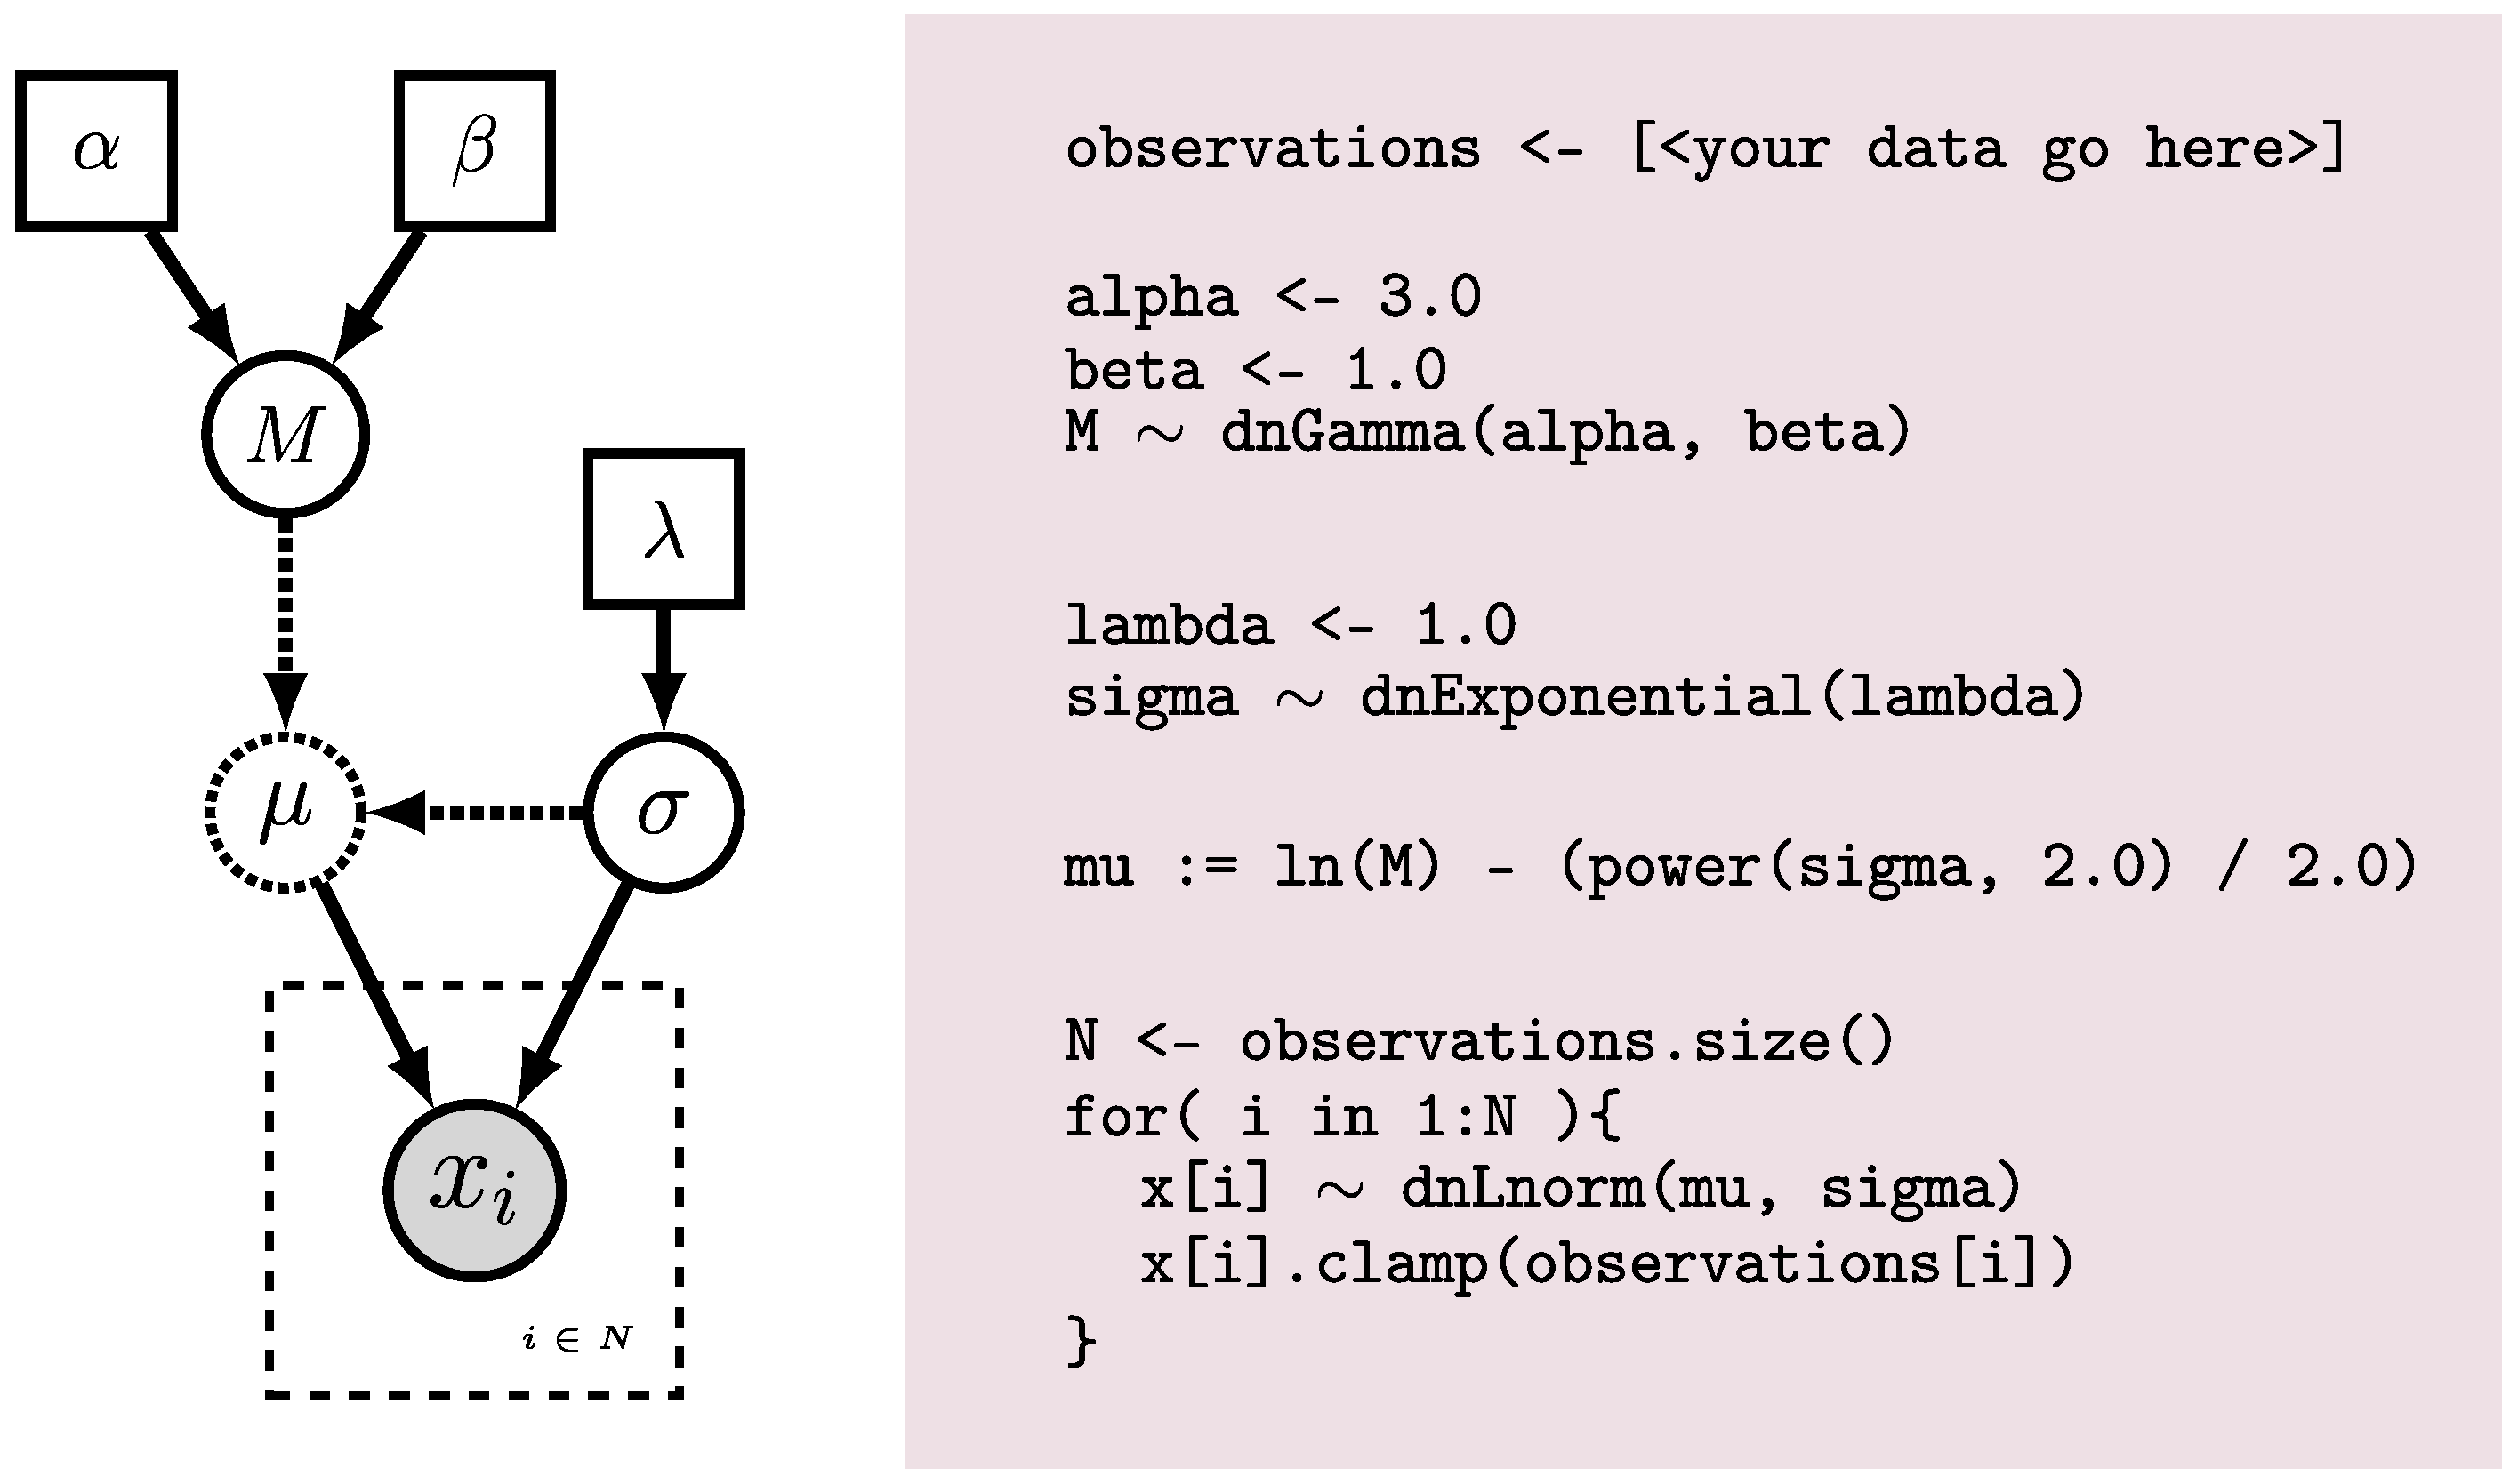
\includegraphics[width=5in,angle=0]{figures/simple_GM_rev.eps}}
\caption{\small Specifying a model in the Rev language. The graphical model of the observed parameter $x$ is shown on the left. 
In this example, $x$ is log-normally distributed with a location parameter of $\mu$ and a standard deviation of 
$\sigma$, thus $x \sim \mbox{Lognormal}(\mu, \sigma)$. The expected value of $x$ (or mean) is equal to $M$: $\mathbb{E}(x) = M$. 
In this model, $M$ and $\sigma$ are random variables and each are assigned hyperpriors. 
We assume that the mean is drawn from a gamma distribution with shape parameter $\alpha$ and rate parameter 
$\beta$: $M \sim \mbox{Gamma}(\alpha, \beta)$. The standard deviation of the lognormal distribution is assigned an 
exponential hyperprior with rate $\lambda$: $\sigma \sim \mbox{Exponential}(\lambda)$. 
Since we are conditioning our model on the \textit{expectation}, we must compute the location parameter ($\mu$) to 
calculate the probability of our model. 
Thus, $\mu$ is a deterministic node that is the result of the function$^*$ executed on $M$ and $\sigma$: $\mu = \ln(M) - \frac{\sigma^2}{2}$. 
Since we observe values of $x$, we \textit{clamp} this node.
{\scriptsize $^*$[Note that a current bug in the language related to nested functions means that \cl{mu := ln(M) - (power(sigma, 2.0) / 2.0)} does not correctly identify the parent nodes of \cl{mu}. To work around this, we need two additional deterministic nodes: \cl{lnM := ln(M)} and \cl{variance := power(sigma, 2.0)}. And \cl{mu} is changed to \cl{mu := lnM - (variance / 2.0)}.]}
}
\label{revgmexample}
\end{figure}

Deterministic nodes are variable transformations and initialized using the \cl{:=} operator followed by the function or formula for calculating the value. 
Thus, if you had an exponentially distributed stochastic node and you also wanted to monitor the square root of that variable, you can create a deterministic node:
{\tt \begin{snugshade*}
\begin{lstlisting}
p ~ dnExponential(1.0)
sq_p := sqrt(p)
\end{lstlisting}
\end{snugshade*}}

Replication over lists of variables as a plate object is specified using \cl{for} loops. 
A for-loop is an iterator statement that performs a function a given number of times. 
In RevBayes you can use this syntax to create a vector of 12 stochastic nodes, each drawn from a Poisson distribution:
{\tt \begin{snugshade*}
\begin{lstlisting}
rate <- 2.5
for( i in 1:12 ){
  p[i] ~ dnPoisson(rate)
}
\end{lstlisting}
\end{snugshade*}}

A clamped node is attached to observed data. Thus, you must first read in or input the data as a constant node, then clamp it to a stochastic node. 
In Figure \ref{revgmexample} the observations are assigned and clamped to the stochastic nodes.
If we observed 7 values for \cl{x} we would create 7 clamped nodes:
{\tt \begin{snugshade*}
\begin{lstlisting}
observations <- [0.20, 0.21, 0.03, 0.40, 0.65, 0.87, 0.22]
N <- observations.size()
for( i in 1:N ){
  x[i] ~ dnLognormal(mu, sigma)
  x[i].clamp(observations.clamp)
}
\end{lstlisting}
\end{snugshade*}}


\vspace{5mm}

{\begin{framed}
\begin{center}
Continue on to the next page to start the exercise...
\end{center}
\end{framed}}



%
%\subsection*{Analysis Functions}
%
\newpage
\FloatBarrier
\section{Exercise: Model Selection \& Partitioning using Bayes Factors}

\subsection{Introduction}
%
%
%\bigskip
%\section{Model Selection \& Partitioning using Bayes Factors}

Variation in the evolutionary process across the sites of nucleotide 
sequence alignments is well established, and is an increasingly pervasive feature of datasets 
composed of gene regions sampled from multiple loci and/or different genomes.
Inference of phylogeny from these data demands that we adequately model the underlying process heterogeneity; 
failure to do so can lead to biased estimates of phylogeny and other parameters \citep{brown07}.
To accommodate process heterogeneity within and/or between various gene(omic)
regions, we will evaluate the support for various partition schemes 
using Bayes factors to compare the marginal likelihoods of the candidate partition schemes.

Accounting for process heterogeneity involves adopting a `mixed-model' approach, \citep{ronquist03} in which the sequence alignment is first parsed into a number of partitions that are intended to capture plausible process heterogeneity within the data.
The determination of the partitioning scheme is guided by biological considerations regarding the dataset at hand.
For example, we might wish to evaluate possible variation in the evolutionary process within a single gene region ({\it e.g.}, between stem and loop regions of ribosomal sequences), or among gene regions in a concatenated alignment ({\it e.g.}, comprising multiple nuclear loci and/or gene regions sampled from different genomes).
The choice of partitioning scheme is up to the investigator and many possible partitions might be considered for a typical dataset.

Next, a substitution model is specified for each predefined process partition (using a given model-selection criterion, such as Bayes factors).
In this exercise, we assume that each partition evolved under an independent general-time reversible model with gamma-distributed rates across sites (GTR+$\Gamma$). 
Under this model the observed data are conditionally dependent on the exchangeability rates ($\theta$), stationary base frequencies ($\pi$), and the degree of gamma-distributed among-site rate variation ($\alpha$), as well as the unrooted tree topology ($\Psi$) and branch lengths ($\nu$).
We show the graphical model representation of the GTR+$\Gamma$ mode in Figure \ref{gtrgmfig}. 
When we assume different GTR+$\Gamma$ models for each partitions, this results in a composite model, in which all sites are assumed to share a common, unrooted tree topology and proportional branch lengths, but subsets of sites (`data partitions') are assumed to have independent substitution model parameters.
This composite model is referred to as a \emph{mixed model}. %\taha{need to change the graphical model above to have the same symbols as in this paragraph since this refers to the figure \ref{pipeline} and it may be harder to change that figure.}



Finally, we perform a separate MCMC simulation to approximate the joint posterior probability density of the phylogeny and other parameters.  Note that, in this approach, the mixed model is a fixed assumption of the inference ({\it i.e.}, the parameter estimates are conditioned on the specified mixed model), and the parameters for each process partition are independently estimated.

For most sequence alignments, several (possibly many) partition schemes of varying complexity are plausible {\it a priori}, which therefore requires a way to objectively identify the partition scheme that balances estimation bias and error variance associated with under- and over-parameterized mixed models, respectively.
Increasingly, mixed-model selection is based on \textit{Bayes factors} \citep[{\it e.g.},][]{suchard01}, which involves first calculating the marginal likelihood under each candidate partition scheme and then comparing the ratio of the marginal likelihoods for the set of candidate partition schemes \citep{brandley05,nylander04,mcguire07}.
The analysis pipeline that we will use in this tutorial is depicted in Figure \ref{pipeline}.
\begin{figure}[h!]
\centering
\fbox{\includegraphics[width=6.8in,angle=0]{figures/pipeline.eps}}
\caption{\small The analysis pipeline for Exercise 1. We will explore three partition schemes for the conifer dataset.
The first model (the `uniform model', $M_0$) assumes that all sites evolved under a common GTR+$\Gamma$ substitution model.
The second model (the `moderately partitioned' model, $M_1$) invokes two data partitions corresponding to the two gene regions (atpB and rbcL), and assumes each subset of sites evolved under an independent GTR+$\Gamma$ model.
The final mixed model (the `highly partitioned' model, $M_2$) invokes four data partitions---the first partition corresponds to the atpB gene region, and the remaining partitions correspond to the three codon positons of the rbcL gene region---and each data partition is assumed evolved under an independent GTR+$\Gamma$ substitution model.
Note that we assume that all sites share a common tree topology, $\Psi$, and branch-length proportions, $\nu$, for each of the candidate partition schemes.
We perform two separate sets of analyses for each mixed model---a Metropolis-coupled MCMC simulation to approximate the joint posterior probability density of the mixed-model parameters, and a `stepping-stone' MCMC simulation to approximate the marginal likelihood for each mixed model.
The resulting marginal-likelihood estimates are then evaluated using Bayes factors to assess the fit of the data to the three candidate mixed models.  
}
\label{pipeline}
\end{figure}
 
Given two models, $M_0$ and $M_1$, the Bayes factor comparison assessing the relative plausibility of each model as an explanation of the data, $BF(M_0,M_1)$, is:
$$BF(M_0,M_1) = \frac{\mbox{posterior odds}}{\mbox{prior odds}}.$$
The posterior odds is the posterior probability of $M_0$ given the data, $\mathbf X$, divided by the posterior odds of $M_1$ given the data:
$$\mbox{posterior odds} = \frac{\mathbb{P}(M_0 \mid \mathbf X)}{\mathbb{P}(M_1 \mid \mathbf X)},$$
and the prior odds is the prior probability of $M_0$ divided by the prior probability of $M_1$:
$$\mbox{prior odds} = \frac{\mathbb{P}(M_0)}{\mathbb{P}(M_1)}.$$
Thus, the Bayes factor measures the degree to which the data alter our belief regarding the support for $M_0$ relative to $M_1$ \citep{lavine99}:
\begin{align}\label{BFeq1}
BF(M_0,M_1) = \frac{\mathbb{P}(M_0 \mid \mathbf X, \theta_0)}{\mathbb{P}(M_1 \mid \mathbf X, \theta_1)} \div \frac{\mathbb{P}(M_0)}{\mathbb{P}(M_1)}. 
\end{align}
This, somewhat vague, definition does not lead to clear-cut identification of the ``best'' model. Instead, \textsl{you} must decide the degree of your belief in $M_0$ relative to $M_1$. 
Despite the absence of any strict ``rule-of-thumb'', you can refer to the scale \citep[outlined by][]{jeffreys61} for interpreting these measures (Table \ref{bftable}).
\begin{table}[h]
\centering
\caption{\small The scale for interpreting Bayes factors by Harold \citet{jeffreys61}.} 
\label{bftable}
\begin{tabular}{l c r}
\hline
\multicolumn{1}{l}{\textbf{$BF(M_0, M_1)$}} & \multicolumn{1}{r}{ } &\multicolumn{1}{r}{{Strength of evidence}} \\ 
\hline
$<1:1$ & \hspace{8mm} & Negative (supports $M_1$)\\
$1:1$ to $3:1$ & & Barely worth mentioning\\
$3:1$ to $10:1$ & & Substantial\\
$10:1$ to $30:1$ & & Strong\\
$30:1$ to $100:1$ & & Very strong\\
$>100:1$ & & Decisive\\
\hline
\multicolumn{3}{l}{{\scriptsize{For a detailed description of Bayes factors see \citet{kass95}}}} 
\end{tabular}
\end{table}


Unfortunately, direct calculation of the posterior odds to prior odds ratio is unfeasible for most phylogenetic models. However, we can further define the posterior odds ratio as:
\begin{align*}
\frac{\mathbb{P}(M_0 \mid \mathbf X)}{\mathbb{P}(M_1 \mid \mathbf X)} = \frac{\mathbb{P}(M_0)}{\mathbb{P}(M_1)} \frac{\mathbb{P}(\mathbf X \mid M_0)}{\mathbb{P}(\mathbf X \mid M_1)},
\end{align*}
where $\mathbb{P}(\mathbf X \mid M_i)$ is the \textit{marginal likelihood} of the data marginalized over all parameters for $M_i$; it is also referred to as the \textit{model evidence} or \textit{integrated likelihood}.
More explicitly, the marginal likelihood is the probability of the set of observed data ($\mathbf X$) under a given model ($M_i$), while averaging over all possible values of the parameters of the model ($\theta_i$) with respect to the prior density on $\theta_i$
\begin{align}\label{margeLike}
\mathbb{P}(\mathbf X \mid M_i) = \int \mathbb{P}(\mathbf X \mid \theta_i) \mathbb{P}(\theta_i)dt.
\end{align}
If you refer back to equation \ref{BFeq1}, you can see that, with very little algebra, the ratio of marginal likelihoods is equal to the Bayes factor:
\begin{align}\label{bfFormula}
BF(M_0,M_1) = \frac{\mathbb{P}(\mathbf X \mid M_0)}{\mathbb{P}(\mathbf X \mid M_1)} = \frac{\mathbb{P}(M_0 \mid \mathbf X, \theta_0)}{\mathbb{P}(M_1 \mid \mathbf X, \theta_1)} \div \frac{\mathbb{P}(M_0)}{\mathbb{P}(M_1)}. 
\end{align}
Therefore, we can perform a Bayes factor comparison of two models by calculating the marginal likelihood for each one. % Simple as pie, right?
Alas, exact solutions for calculating marginal likelihoods are not known for phylogenetic models (see equation \ref{margeLike}), thus we must resort to numerical integration methods to estimate or approximate these values. 
In this exercise, we will estimate the marginal likelihood for each partition scheme
using both the stepping-stone \citep{xie11} and path sampling estimators \citep{gelman1998,lartillot06, friel2008}. 


\bigskip
\subsection{Phylogenetic Models}\label{secUnif} 

The models we use here are equivalent to the models described in the previous exercise on MCMC methods and convergence assessment.
To specify the model please consult the previous exercise.


\bigskip
{\large \textcolor{mycol}{\textsc{Estimating the Marginal Likelihood}}}

Typically, model comparison is performed prior to running the full MCMC analysis under a model. 
If you calculated the Bayes factors to determine the relative support for the uniform model and found that there was strong evidence supporting this model over others (hint: this is not true if you proceed with this tutorial), then it would be worth your time to proceed with the MCMC steps outlined above. 
The following steps will describe using stepping-stone and path sampling methods on a set of power posteriors to estimate marginal likelihoods under the uniform model. 

With a fully specified model, we can set up the \cl{powerPosterior()} analysis to create a file of `powers' and likelihoods from which we can estimate the marginal likelihood using stepping-stone or path sampling. 
This method computes a vector of powers from a beta distribution, then executes an MCMC run for each power step while raising the likelihood to that power. In this implementation, the vector of powers starts with 1, sampling the likelihood close to the posterior and incrementally sampling closer and closer to the prior as the power decreases. 



%\textbf{\textit{Clear Workspace and Load the Data and Model}}

Just to be safe, it is better to clear the workspace and re-load the data and model:
{\tt \begin{snugshade*}
\begin{lstlisting}
RevBayes > clear()
RevBayes > source("RevBayes_scripts/uniform_partition_model.Rev")
\end{lstlisting}
\end{snugshade*}}


First, we create the variable containing the power posterior. 
This requires us to provide a model and vector of moves, as well as an output file name. 
The \cl{cats} argument sets the number of power steps.
{\tt \begin{snugshade*}
\begin{lstlisting}
RevBayes > pow_p <- powerPosterior(mymodel, moves, "pow_p_PS0.out", cats=50) 
\end{lstlisting}
\end{snugshade*}}

We can start the power posterior by first burning in the chain and and discarding the first 10000 states.  
{\tt \begin{snugshade*}
\begin{lstlisting}
RevBayes > pow_p.burnin(generations=10000,tuningInterval=1000)
\end{lstlisting}
\end{snugshade*}}

Now execute the run with the \cl{.run()} function:
{\tt \begin{snugshade*}
\begin{lstlisting}
RevBayes > pow_p.run(generations=1000)  
\end{lstlisting}
\end{snugshade*}}

Once the power posteriors have been saved to file, create a stepping stone sampler. 
This function can read any file of power posteriors and compute the marginal likelihood using stepping-stone sampling. 
{\tt \small \begin{snugshade*}
\begin{lstlisting}
RevBayes > ss <- steppingStoneSampler(file="pow_p_PS0.out", powerColumnName="power", likelihoodColumnName="likelihood")
\end{lstlisting}
\end{snugshade*}}

Compute the marginal likelihood under stepping-stone sampling using the member function \cl{marginal()} of the \cl{ss} variable and record the value in Table \ref{ssTable}.
{\tt \begin{snugshade*}
\begin{lstlisting}
RevBayes > ss.marginal() 
\end{lstlisting}
\end{snugshade*}}

Path sampling is an alternative to stepping-stone sampling and also takes the same power posteriors as input. 
{\tt \small \begin{snugshade*}
\begin{lstlisting}
RevBayes > ps <- pathSampler(file="pow_p_PS0.out", powerColumnName="power", likelihoodColumnName="likelihood")
\end{lstlisting}
\end{snugshade*}}

Compute the marginal likelihood under stepping-stone sampling using the member function \cl{marginal()} of the \cl{ps} variable and record the value in Table \ref{ssTable}.
{\tt \begin{snugshade*}
\begin{lstlisting}
RevBayes > ps.marginal() 
\end{lstlisting}
\end{snugshade*}}


Repeat this analysis for each of the other three partitioning schemes.




\bigskip
\subsection{Compute Bayes Factors and Select Model}


Now that we have estimates of the marginal likelihood under each of our different models, we can evaluate their relative plausibility using Bayes factors.
Use Table \ref{ssTable} to summarize the marginal log-likelihoods estimated using the stepping-stone and path-sampling methods.
\begin{Form}
\begin{table}[h]
\centering
\caption{\small Estimated marginal likelihoods for different partition configurations$^*$.}
\begin{tabular}{l c c c c}
\hline
\multicolumn{1}{l}{\textbf{ }} &\multicolumn{1}{r}{\textbf{ }} & \multicolumn{3}{c}{\textbf{Marginal lnL estimates}} \\ 
\cline{3-5}
\multicolumn{1}{l}{\textbf{Partition}} & \multicolumn{1}{r}{\hspace{3mm}} & \multicolumn{1}{c}{\textit{Stepping-stone}} & \multicolumn{1}{r}{\hspace{3mm}} & \multicolumn{1}{c}{\textit{Path sampling}} \\ 
\hline
uniform ($M_1$) & \hspace{15mm} & \TextField[name=m1,backgroundcolor={.85 .85 .85},color={1 0 0},height=4ex]{}  & \hspace{15mm} & \TextField[name=ml2,backgroundcolor={.85 .85 .85},color={0 0 1},height=4ex]{} \\
\hline
by gene ($M_2$) & \hspace{3mm} &\TextField[name=ml3,backgroundcolor={.85 .85 .85},color={1 0 0},height=4ex]{}   & \hspace{3mm} & \TextField[name=ml4,backgroundcolor={.85 .85 .85},color={0 0 1},height=4ex]{} \\
\hline
linked codons ($M_3$) & \hspace{3mm} &\TextField[name=ml3,backgroundcolor={.85 .85 .85},color={1 0 0},height=4ex]{}   & \hspace{3mm} & \TextField[name=ml4,backgroundcolor={.85 .85 .85},color={0 0 1},height=4ex]{} \\
\hline
saturated ($M_4$) & \hspace{3mm} & \TextField[name=ml5,backgroundcolor={.85 .85 .85},color={1 0 0},height=4ex]{} & \hspace{3mm} & \TextField[name=ml6,backgroundcolor={.85 .85 .85},color={0 0 1},height=4ex]{} \\
\hline
{\footnotesize{$^*$you can edit this table}}\\
\end{tabular}
\label{ssTable}
\end{table}
\end{Form}

Phylogenetics software programs log-transform the likelihood to avoid \href{http://en.wikipedia.org/wiki/Arithmetic_underflow}{underflow}, because multiplying likelihoods results in numbers that are too small to be held in computer memory.
Thus, we must use a different form of equation \ref{bfFormula} to calculate the ln-Bayes factor (we will denote this value $\mathcal{K}$):
\begin{align}\label{LNbfFormula}
\mathcal{K}=\ln[BF(M_0,M_1)] = \ln[\mathbb{P}(\mathbf X \mid M_0)]-\ln[\mathbb{P}(\mathbf X \mid M_1)],
\end{align}
where $\ln[\mathbb{P}(\mathbf X \mid M_0)]$ is the \textit{marginal lnL} estimate for model $M_0$. 
The value resulting from equation \ref{LNbfFormula} can be converted to a raw Bayes factor by simply taking the exponent of $\cal{K}$
\begin{align}\label{LNbfFormula2}
BF(M_0,M_1) = e^{\cal{K}}.
\end{align}
Alternatively, you can interpret the strength of evidence in favor of $M_0$ using the $\cal{K}$ and skip equation \ref{LNbfFormula2}. 
In this case, we evaluate the $\cal{K}$ in favor of model $M_0$ against model $M_1$ so that:
\begin{center}
\begin{tabular}{l}
if $\mathcal{K} > 1$, then model $M_0$ wins\\
if $\mathcal{K} < -1$, then model $M_1$ wins.
\end{tabular}
\end{center}
Thus, values of $\mathcal{K}$ around 0 indicate ambiguous support. 

%Alternatively, you can refer to a different scale for interpreting the $\ln[BF(M_0,M_1)]$ described by \citet{kass95}.
%\begin{table}[h]
%\centering
%\caption{\small The scale for interpreting $log_e$ Bayes factors by \citet{kass95}.} 
%\begin{tabular}{l c r}
%\hline
%\multicolumn{1}{l}{\textbf{$2\ln[BF(M_0, M_1)]$}} & \multicolumn{1}{r}{ } &\multicolumn{1}{r}{{Strength of evidence \textit{against} $M_0$}} \\ 
%\hline
%0 to 2 & \hspace{8mm} & Not worth more than a bare mention\\
%2 to 6 & \hspace{8mm} & Positive\\
%6 to 10 & \hspace{8mm} & Strong\\
%$>10$ & \hspace{8mm} & Very strong\\
%\hline
%\end{tabular}
%\label{bftable2}
%\end{table}



Using the values you entered in Table \ref{ssTable} and equation \ref{LNbfFormula},  calculate the ln-Bayes factors (using $\mathcal{K}$) for the different model comparisons. 
Enter your answers in Table \ref{bfTable} using the stepping-stone and the path-sampling estimates of the marginal log likelihoods. 

\begin{Form}
\begin{table}[h!]
\centering
\caption{\small Bayes factor calculation$^*$.}
\begin{tabular}{l c c c c}
\hline
\multicolumn{1}{l}{\textbf{ }} &\multicolumn{1}{r}{\textbf{ }} & \multicolumn{3}{c}{\textbf{ln-Bayes Factor} ($\mathcal{K}$)} \\ 
\cline{3-5}
\multicolumn{1}{l}{\textbf{Model comparison}} & \multicolumn{1}{r}{\hspace{3mm}} & \multicolumn{1}{c}{\textit{Stepping-stone}} & \multicolumn{1}{r}{\hspace{3mm}} & \multicolumn{1}{c}{\textit{Path sampling}} \\ 
\hline
$M_1,M_2$ & \hspace{15mm} & \TextField[name=ml7,backgroundcolor={.85 .85 .85},color={1 0 0},height=4ex]{}  & \hspace{15mm} & \TextField[name=ml8,backgroundcolor={.85 .85 .85},color={0 0 1},height=4ex]{} \\
\hline
$M_1,M_3$ & \hspace{3mm} &  \TextField[name=ml11,backgroundcolor={.85 .85 .85},color={1 0 0},height=4ex]{} & \hspace{3mm} & \TextField[name=ml12,backgroundcolor={.85 .85 .85},color={0 0 1},height=4ex]{} \\
\hline
$M_1,M_4$ & \hspace{3mm} & \TextField[name=ml9,backgroundcolor={.85 .85 .85},color={1 0 0},height=4ex]{} & \hspace{3mm} & \TextField[name=ml10,backgroundcolor={.85 .85 .85},color={0 0 1},height=4ex]{} \\
\hline
$M_2,M_3$ & \hspace{3mm} & \TextField[name=ml9,backgroundcolor={.85 .85 .85},color={1 0 0},height=4ex]{} & \hspace{3mm} & \TextField[name=ml10,backgroundcolor={.85 .85 .85},color={0 0 1},height=4ex]{} \\
\hline
$M_2,M_4$ & \hspace{3mm} & \TextField[name=ml9,backgroundcolor={.85 .85 .85},color={1 0 0},height=4ex]{} & \hspace{3mm} & \TextField[name=ml10,backgroundcolor={.85 .85 .85},color={0 0 1},height=4ex]{} \\
\hline
$M_3,M_4$ & \hspace{3mm} & \TextField[name=ml9,backgroundcolor={.85 .85 .85},color={1 0 0},height=4ex]{} & \hspace{3mm} & \TextField[name=ml10,backgroundcolor={.85 .85 .85},color={0 0 1},height=4ex]{} \\
\hline
Supported model? & \hspace{3mm} &  \TextField[name=ml13,backgroundcolor={1 .85 .85},color={1 0 0},height=4ex]{} & \hspace{3mm} & \TextField[name=ml14,backgroundcolor={.85 .85 1},color={0 0 1},height=4ex]{} \\
\hline
{\footnotesize{$^*$you can edit this table}}\\
\end{tabular}
\label{bfTable}
\end{table}
\end{Form}

%Once you complete Table \ref{bfTable}, you will notice that the Bayes factor comparison indicates strong evidence in support of the highly partitioned model using both the stepping-stone and path sampling estimates of the marginal likelihoods. 
%However, this does not mean that model $M_3$ is the \textit{true} partition model.
%We only considered three out of the many, many possible partitions for 2,659 sites (the number of possible partitions can be viewed if you compute the \href{http://www.wolframalpha.com/input/?i=bell+number(2659)}{$2659^{th}$ Bell number}). 
%Given the strength of support for the highly partitioned model, it is possible that further partitioning is warranted for these data. 
%In particular, partitioning the dataset by codon position for both atpB \textit{and} rbcL is an important next step for this exercise (consider taking some time on your own to test this model). 

Because of the computational costs of computing marginal likelihoods and the vast number of possible partitioning strategies, it is not feasible to evaluate all of them. 
New methods based on nonparametric Bayesian models have recently been applied to address this problem \citep{lartillot04,huelsenbeck07b,wuCH2013}. 
These approaches use an infinite mixture model \citep[the Dirichlet process;][]{ferguson73,antoniak74} that places non-zero probability on \textit{all} of the countably-infinite possible partitions for a set of sequences. 
Bayesian phylogenetic inference under these models is implemented in the program \href{http://megasun.bch.umontreal.ca/People/lartillot/www/index.htm}{PhyloBayes} \citep{Lartillot2009} and the \href{https://code.google.com/p/subst-bma/}{subst-bma} plug-in for \href{http://beast2.cs.auckland.ac.nz/index.php/Main_Page}{BEAST2} \citep{wuCH2013}.


% $$B_{1,2} = e^{ln(B_{12})}$$
% $$ln(MlnL_1) - ln(MlnL_2)$$

%When you complete Table \ref{bfTable} and evaluate the Bayes factors using \citet{jeffreys61} scale in Table \ref{bftable}, you will notice that no single model model stands out as ``strongly supported''. 
%Every Bayes factor comparison is ``barely worth mentioning''. 

Note that Bayes factors based on comparison of HM-based marginal likelihoods 
often \textit{strongly} favor the most extremely partitioned mixed model. 
In fact, the harmonic mean estimator has been shown to provide unreliable estimates of marginal likelihoods, compared to more robust approaches \citep{lartillot06,xie11,fan11}.
Based on these studies, it is recommended that you avoid %never, ever, ever
using HM-derived marginal likelihoods for Bayes factor comparisons.
%base Bayes factors on comparisons of HM-derived marginal likelihoods. 
(The Canadian Bayesian Radford Neal says the harmonic mean is the ``\href{http://radfordneal.wordpress.com/2008/08/17/the-harmonic-mean-of-the-likelihood-worst-monte-carlo-method-ever/}{worst Monte Carlo method ever}''.)


\vspace{5cm}
Questions about this tutorial can be directed to: \\\vspace{-10mm}
\begin{itemize}
\item Tracy Heath (email: \href{mailto:tracyh@berkeley.edu}{tracyh@berkeley.edu}) \\\vspace{-8mm}
\item Michael Landis (email: \href{mailto:mlandis@berkeley.edu}{mlandis@berkeley.edu}) \\\vspace{-8mm} 
\item Sebastian H\"{o}hna (email: \href{mailto:sebastian.hoehna@gmail.com}{sebastian.hoehna@gmail.com})
\end{itemize}

\href{http://creativecommons.org/licenses/by/4.0/}{
\includegraphics[scale=0.8]{figures/ccby.eps}} This tutorial was written by \href{http://phylo.bio.ku.edu/content/tracy-heath}{Tracy Heath}, \href{http://michaeljameslandis.com/}{Michael Landis}, and Sebastian H\"{o}hna; licensed under a \href{http://creativecommons.org/licenses/by/4.0/}{Creative Commons Attribution 4.0 International License}. 
(This tutorial is based on the \href{http://treethinkers.org/tutorials/phylogenetic-inference-using-mrbayes-v3-2/}{Phylogenetic Inference using MrBayes v3.2} tutorial written by Tracy Heath, Conor Meehan, and Brian Moore and some content is reproduced here.
Mark Holder, Ben Liebeskind, Emily McTavish, and April Wright provided helpful comments.)

Version dated: \today


{\renewcommand{\bibsection}{\section*{Relevant References}}


\bibliography{bib_tex/master_refs}




\end{document}
